\documentclass[12pt,a4paper]{article}
\usepackage[utf8]{inputenc}
\usepackage[spanish]{babel}
\usepackage{amsmath}
\usepackage{amsfonts}
\usepackage{amssymb}
\usepackage{graphicx}
\usepackage[left=2cm,right=2cm,top=2cm,bottom=2cm]{geometry}
\usepackage{float}
\usepackage{caption}
\usepackage{subcaption}
\author{Carlos Alonso Aznarán Laos}
\title{Práctica N$^{\circ}$4}

\begin{document}
\maketitle

\section{Gráficos con \texttt{includegraphics}}

\includegraphics[scale=0.5]{logo_unii}

\section{Gráficos usando el entorno \texttt{figure}}

\begin{figure}[h]
\centering
\hspace{4.5cm}
\includegraphics[scale=1]{escud_mati}
\label{UNI}
\vspace{-1cm}
\caption{Escudo de la UNMSM}
		
\end{figure}

\pagebreak

\section{Gráfico 1}
\includegraphics[scale=0.5]{PUCP_4}

\section{Gráfico 2}
\includegraphics[scale=0.5]{logo_uta}
\section{Gráfico 3}
\includegraphics[scale=1]{logo_FCEN}
\pagebreak
\section{Ejemplos EPS - PostScript encapsulado}


\begin{figure}[h]
\begin{subfigure}[b]{0.3 \textwidth} 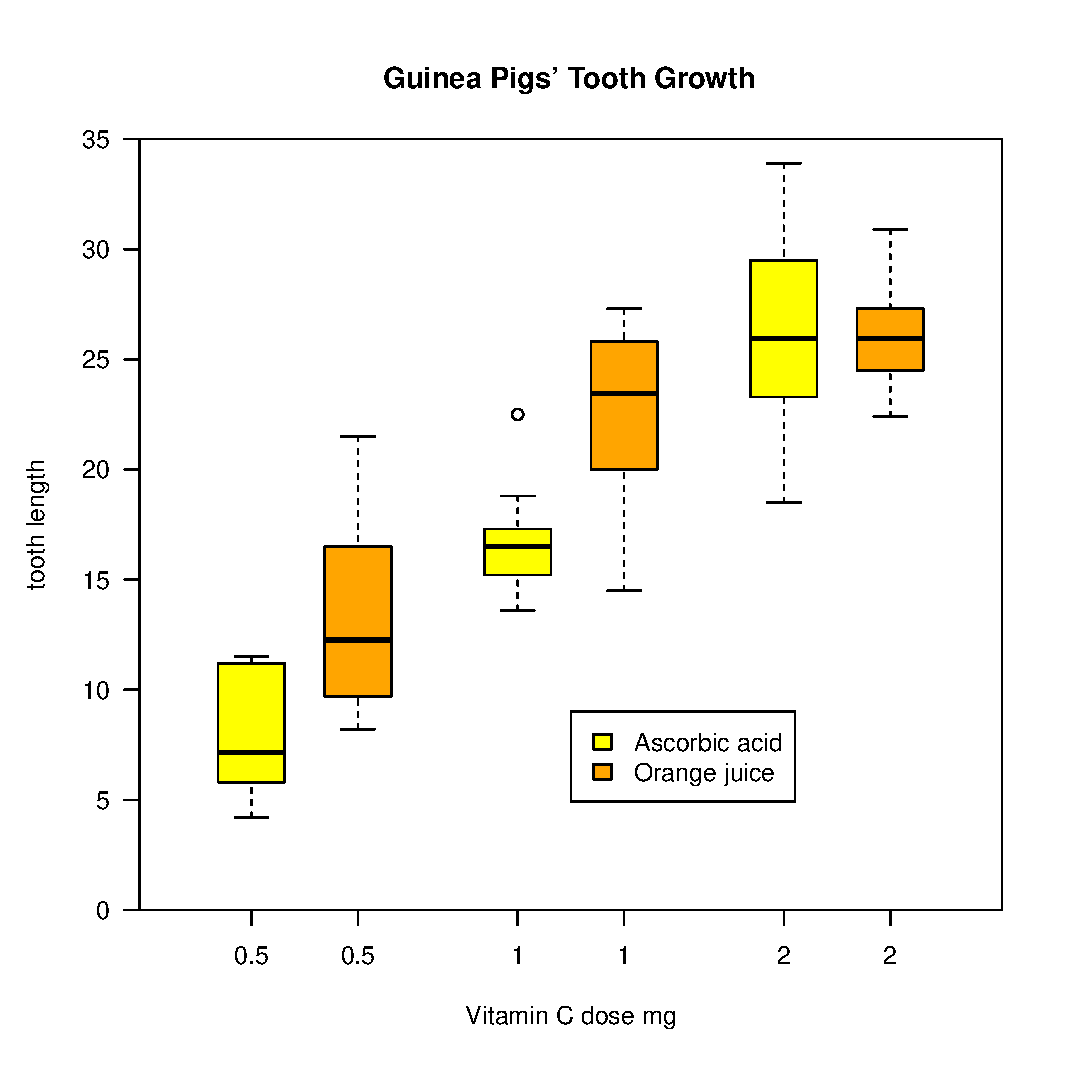
\includegraphics[width=\textwidth]{boxplot} \caption{Dispersion}
\label{fig:disp}
\end{subfigure}
~
\begin{subfigure}[b]{0.3 \textwidth} 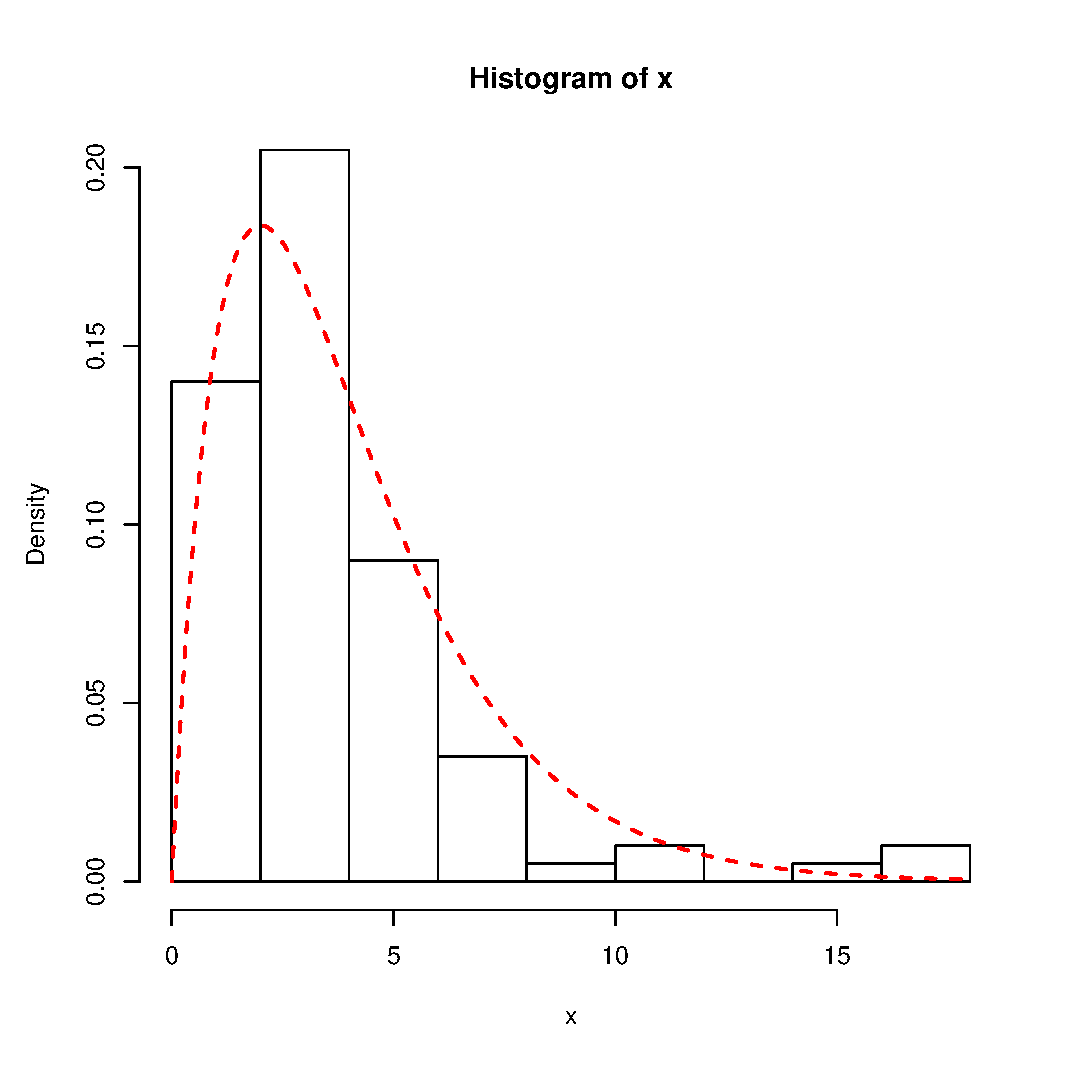
\includegraphics[width=\textwidth]{histograma} \caption{Histograma}
\label{fig:hist}
\end{subfigure}
~
\begin{subfigure}[b]{0.3 \textwidth} 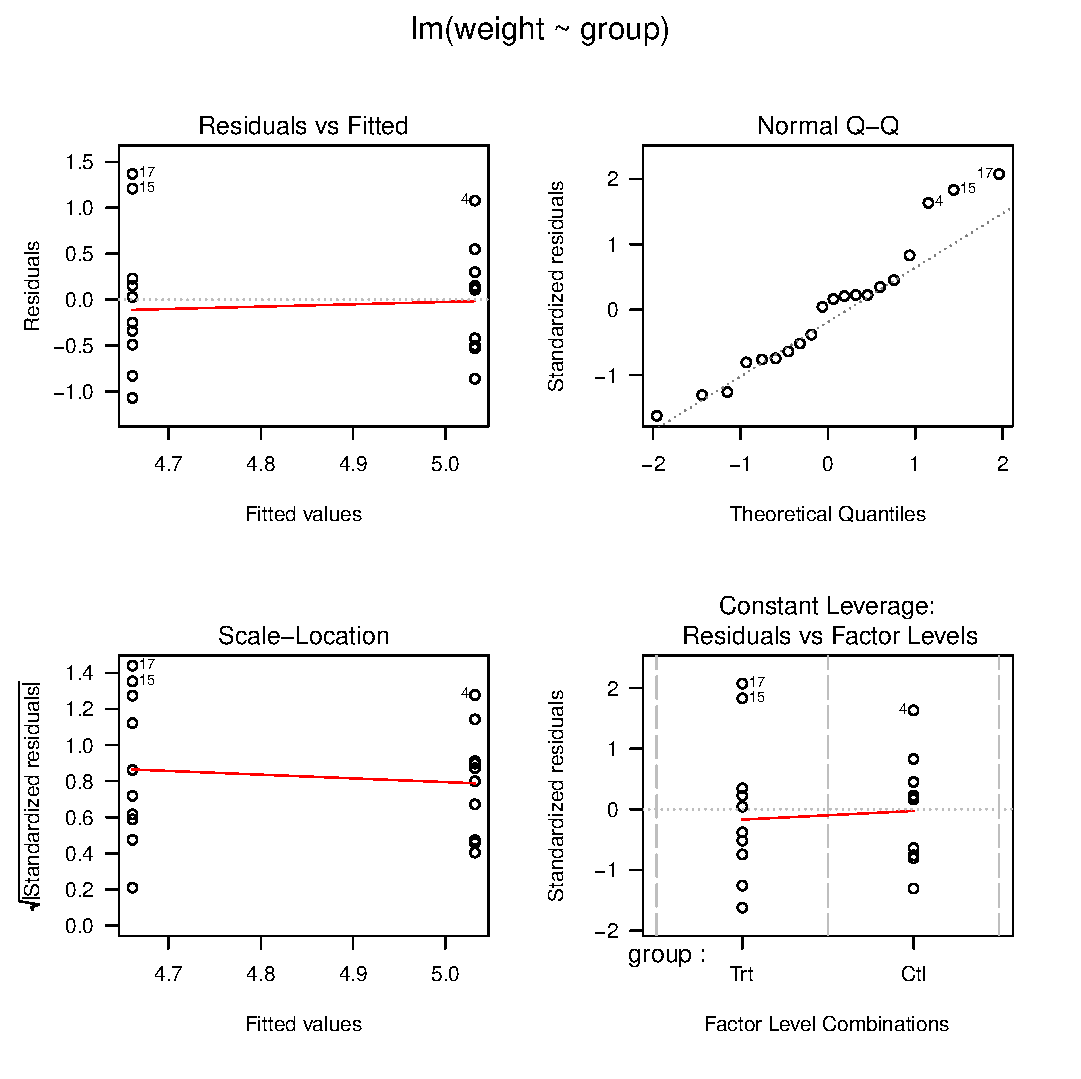
\includegraphics[width=\textwidth]{residuos} \caption{Residuos}
\label{fig:resid}
\end{subfigure}
\caption{Tipos de gráficos}
\label{fig:graf}
\end{figure}
\end{document}